
\documentclass[10pt,a4paper]{article}
\usepackage[utf8]{inputenc}
\usepackage[english]{babel}
%\usepackage{minted}
\usepackage{listings}
\usepackage{xcolor}
\usepackage{graphicx}

%For syntax highlighting
\definecolor{codegreen}{rgb}{0,0.6,0}
\definecolor{codegray}{rgb}{0.5,0.5,0.5}
\definecolor{codepurple}{rgb}{0.58,0,0.82}
\definecolor{backcolour}{rgb}{1,1,1}

%%Sets different parameters
\lstdefinestyle{mystyle}{
	backgroundcolor=\color{backcolour},   
    commentstyle=\color{codegreen},
    keywordstyle=\color{magenta},
    numberstyle=\tiny\color{codegray},
    stringstyle=\color{codepurple},
    basicstyle=\ttfamily\footnotesize,
    breakatwhitespace=false,         
    breaklines=true,                 
    captionpos=b,                    
    keepspaces=true,                 
    numbers=left,                    
    numbersep=5pt,                  
    showspaces=false,                
    showstringspaces=false,
    showtabs=false,                  
    tabsize=4
}
\lstset{style=mystyle}

\title{\bf Matrix Operations, Sorting, BCD Arithmetic}
\author{\vspace{-10ex}}
\date{\vspace{-10ex}}
\begin{document}
\maketitle

\begin{minipage}{0.45\textwidth}
        \begin{tabular}{l l}
            \textbf{Expt No:}&5, 6, 7\\
            \textbf{Date :}&09/10/2020
        \end{tabular}
\end{minipage}%
\begin{minipage}{0.45\textwidth}
        \begin{tabular}{l l}
             \textbf{Name:}& Shivanirudh S G  \\
             \textbf{Reg No:} & 185001146 
        \end{tabular}
\end{minipage}
\vspace{1cm}
\hrule


\begin{flushleft}
\section*{\textbf{Ex 5: Matrix Operations}}
\subsection*{\textbf{Aim:}} 
To perform matrix operations in 8086.

\vspace{1cm}
\hrule
\subsection*{\textbf{\underline{Matrix Addition}}}

\subsubsection*{\textbf{Algorithm:}}
\begin{itemize}
    \item Move the data segment to the AX register and then move it to the DS register.
    \item Move offsets of mat1, mat2 and mat3 into SI, DI, BX registers respectively.
    \item Move value of count to CX register
    \item Move values of r1, r2, c1, c2 into AL, AH, DL, DH registers respectively. 
    \item Compare AL, AH by CMP AL, AH and jump to exit if unequal.
    \item Compare BL, BH by CMP BL, BH and jump to exit if unequal.
    \item Move value at [SI] to AL register.
    \item Add AL with value at [DI].
    \item Move value at AL to [BX].
    \item Increment SI, DI and BX, decrease CX, repeat till CX = 0.
\end{itemize}

\newpage
\subsubsection*{\textbf{Program:}}

\begin{table}[htb]
\centering
\resizebox{\columnwidth}{!}{
\begin{tabular}{|l|l|} 
\hline
\textbf{Program}                                                 & \textbf{Comments}                             \\ 
\hline
\hline
assume cs:code, ds:data                                          & Declare code and data segments                \\
\hline
data segment                                                     & Start of data segment                         \\
\hline
r1 db 02H                                                        & Define byte r1 with value 02H                 \\
\hline 
r2 db 02H                                                        & Define byte r2 with value 02H                 \\
\hline
c1 db 03H                                                        & Define byte c1 with value 03H                 \\
\hline
c2 db 03H                                                        & Define byte c2 with value 03H                 \\
\hline
count dw 0006H                                                   & Define word count with value 0006H            \\
\hline
mat1 db 22H, 33H, 44H, 55H, 66H, 77H                             & Define matrix of values mat1                  \\
\hline
mat2 db 33H, 44H, 55H, 66H, 77H, 88H                             & Define matrix of values mat2                  \\
\hline 
mat3 db ?                                                        & Define result matrix of values mat3           \\
\hline
data ends                                                        & End of data segment                           \\
\hline
code segment                                                     & Start of code segment                         \\
\hline
start:~mov ax, data                                              & Move data to AX register                      \\
\hline
mov ds, ax                                                       & Move contents of AX register to DS register   \\
\hline
mov dl, 0AH                                                      & Move hex value 0A to DL register              \\
\hline
mov si, offset mat1                                              & Move offset of mat1 to SI register            \\
\hline
mov di, offset mat2                                              & Move offset of mat2 to DI register            \\
\hline
mov bx, offset mat3                                              & Move offset of mat3 to BX register            \\
\hline
mov cx, count                                                    & Move value of count to CX register            \\
\hline
mov al, r1                                                       & Move value of r1 to AL register               \\
\hline
mov ah, r2                                                       & Move value of r2 to AH register               \\
\hline
mov dl, c1                                                       & Move value of c1 to DL register               \\
\hline
mov dh, c2                                                       & Move value of c2 to DH register               \\ 
\hline
cmp al, ah                                                       & Compare values of AL and AH registers         \\
\hline
jne exit                                                         & Jump to exit if ZF = 0                        \\
\hline
cmp dl, dh                                                       & Compare values of DL, DH registers            \\
\hline
jne exit                                                         & Jump to exit if ZF = 0                        \\
\hline
here:~mov al, [si]                                               & Move contents at SI to AL register            \\
\hline            
add al, [di]                                                     & AL = AL + [DI]                                \\
\hline
mov [bx], al                                                     & Move contents of AL register to BX register   \\
\hline
inc si                                                           & Increment value in SI register                \\
\hline 
inc di                                                           & Increment value in DI register                \\
\hline
inc bx                                                           & Increment value in BX register                \\         
\hline
dec cx                                                           & Decrement value of CX register                \\
\hline
jnz here                                                         & Jump to here if ZF = 0                        \\
\hline
exit:~mov ah, 4ch                                                & To request interrupt                          \\
\hline
int 21h                                                          & Request interrupt routine                     \\ 
\hline
code ends                                                        & End of code segment                           \\
\hline
end start                                                        &                                               \\
\hline
\end{tabular}
}
\end{table}

\newpage
\subsection*{\textbf{Unassembled code:}}
\begin{figure}[h]
    \centering
    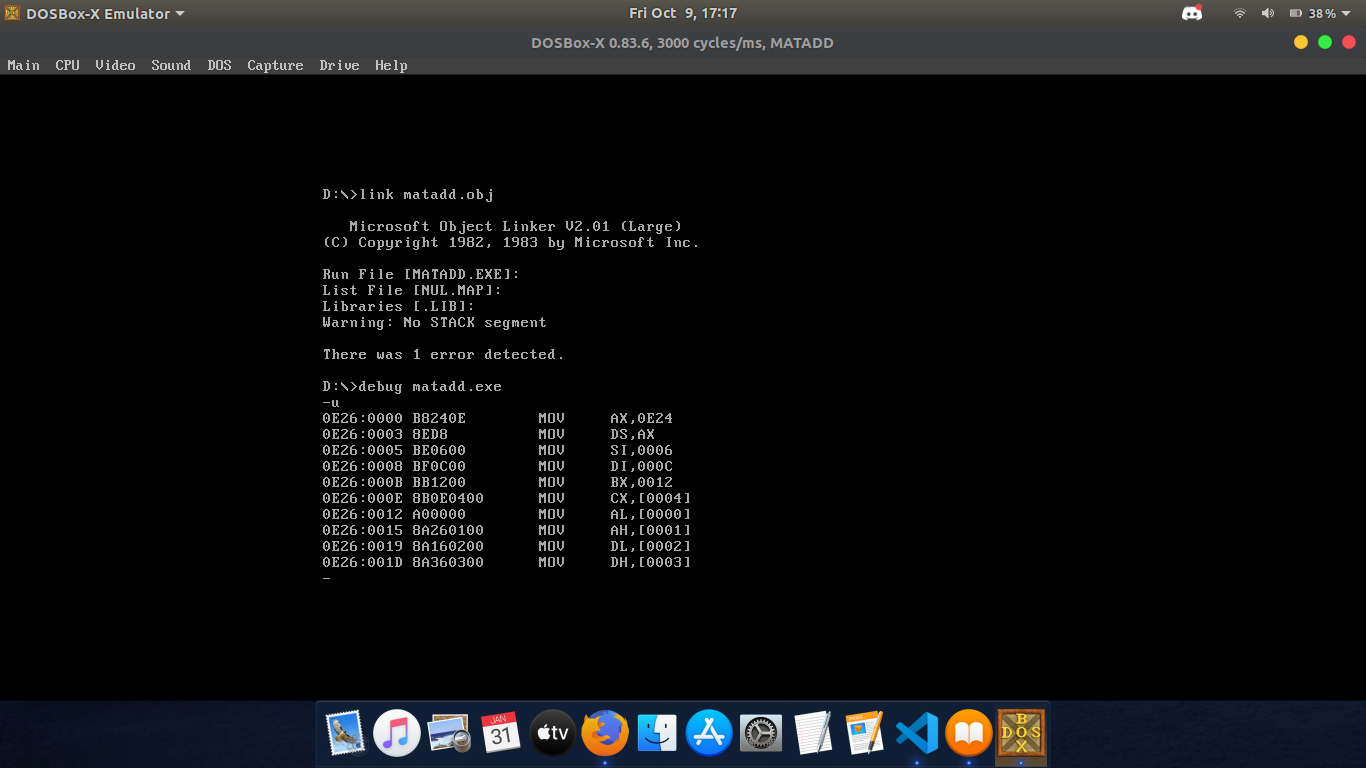
\includegraphics[trim = 100mm 60mm 200mm 120mm, clip, width = \textwidth]{Pics/MAUS.png}
\end{figure}
\subsubsection*{\textbf{Input and Output:}}
\begin{figure}[h]
    \centering
    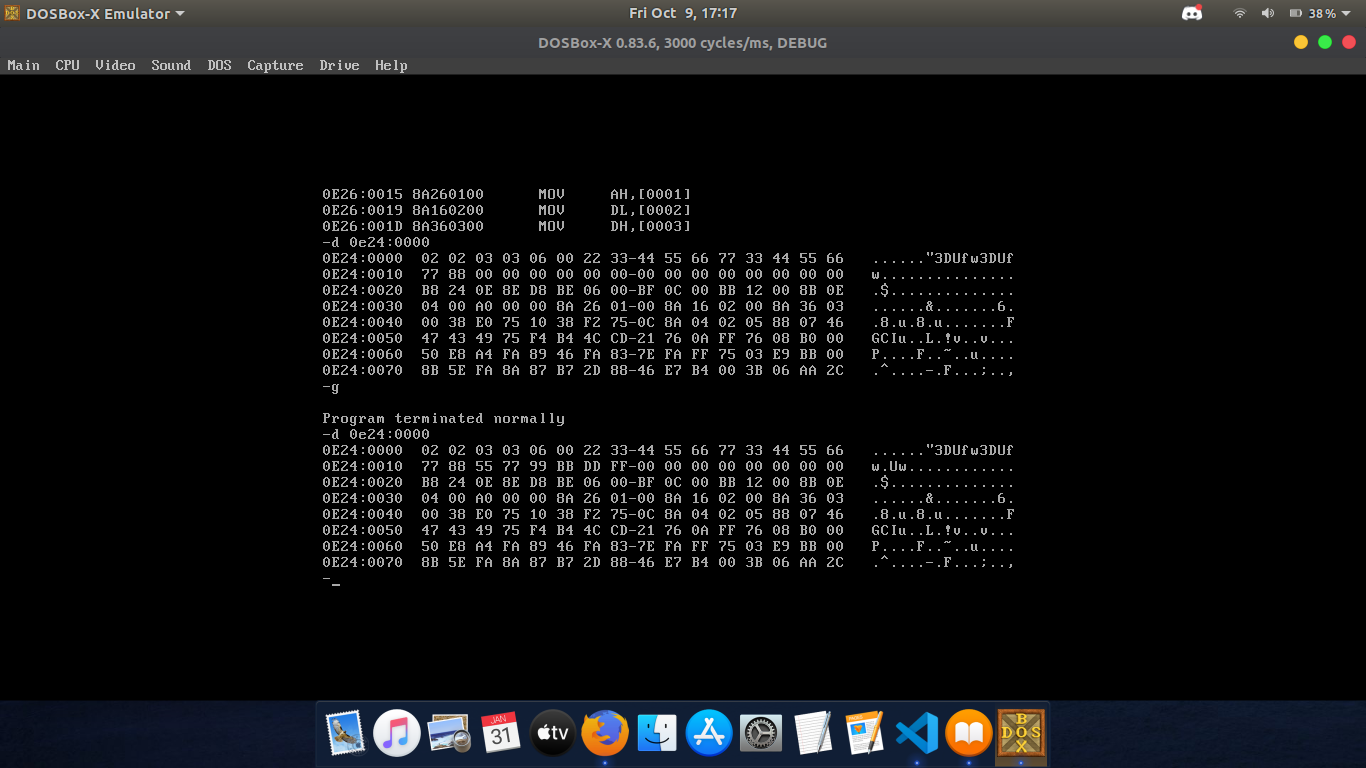
\includegraphics[trim = 100mm 60mm 100mm 80mm, clip, width = \textwidth]{Pics/MAIO.png}
    \caption{ \textbf{Input:} \emph{mat1:} 22H, 33H, 44H, 55H, 66H, 77H; \emph{mat2:} 33H, 44H, 55H, 66H, 77H, 88H ; \newline \hspace{1cm}
              \textbf{Output:} \emph{mat3:} 55H, 77H, 99H, BBH, DDH, FFH}
\end{figure}
%-------------------------------------------------------------------------------------------------------------------------------------------
\hrule
\newpage
\subsection*{\textbf{\underline{Matrix Subtraction}}}

\subsubsection*{\textbf{Algorithm:}}
\begin{itemize}
    \item Move the data segment to the AX register and then move it to the DS register.
    \item Move offsets of mat1, mat2 and mat3 into SI, DI, BX registers respectively.
    \item Move value of count to CX register
    \item Move values of r1, r2, c1, c2 into AL, AH, DL, DH registers respectively. 
    \item Compare AL, AH by CMP AL, AH and jump to exit if unequal.
    \item Compare BL, BH by CMP BL, BH and jump to exit if unequal.
    \item Move value at [DI] to AL register.
    \item Subtract AL with value at [SI].
    \item Move value at AL to [BX].
    \item Increment SI, DI and BX, decrease CX, repeat till CX = 0.
\end{itemize}

\newpage
\subsubsection*{\textbf{Program:}}

\begin{table}[htb]
\centering
\resizebox{\columnwidth}{!}{
\begin{tabular}{|l|l|} 
\hline
\textbf{Program}                                                 & \textbf{Comments}                             \\ 
\hline
\hline
assume cs:code, ds:data                                          & Declare code and data segments                \\
\hline
data segment                                                     & Start of data segment                         \\
\hline
r1 db 02H                                                        & Define byte r1 with value 02H                 \\
\hline 
r2 db 02H                                                        & Define byte r2 with value 02H                 \\
\hline
c1 db 03H                                                        & Define byte c1 with value 03H                 \\
\hline
c2 db 03H                                                        & Define byte c2 with value 03H                 \\
\hline
count dw 0006H                                                   & Define word count with value 0006H            \\
\hline
mat1 db 22H, 33H, 44H, 55H, 66H, 77H                             & Define matrix of values mat1                  \\
\hline
mat2 db 33H, 44H, 55H, 66H, 77H, 88H                             & Define matrix of values mat2                  \\
\hline 
mat3 db ?                                                        & Define result matrix of values mat3           \\
\hline
data ends                                                        & End of data segment                           \\
\hline
code segment                                                     & Start of code segment                         \\
\hline
start:~mov ax, data                                              & Move data to AX register                      \\
\hline
mov ds, ax                                                       & Move contents of AX register to DS register   \\
\hline
mov dl, 0AH                                                      & Move hex value 0A to DL register              \\
\hline
mov si, offset mat1                                              & Move offset of mat1 to SI register            \\
\hline
mov di, offset mat2                                              & Move offset of mat2 to DI register            \\
\hline
mov bx, offset mat3                                              & Move offset of mat3 to BX register            \\
\hline
mov cx, count                                                    & Move value of count to CX register            \\
\hline
mov al, r1                                                       & Move value of r1 to AL register               \\
\hline
mov ah, r2                                                       & Move value of r2 to AH register               \\
\hline
mov dl, c1                                                       & Move value of c1 to DL register               \\
\hline
mov dh, c2                                                       & Move value of c2 to DH register               \\ 
\hline
cmp al, ah                                                       & Compare values of AL and AH registers         \\
\hline
jne exit                                                         & Jump to exit if ZF = 0                        \\
\hline
cmp dl, dh                                                       & Compare values of DL, DH registers            \\
\hline
jne exit                                                         & Jump to exit if ZF = 0                        \\
\hline
here:~mov al, [di]                                               & Move contents at DI to AL register            \\
\hline            
add al, [si]                                                     & AL = AL - [SI]                                \\
\hline
mov [bx], al                                                     & Move contents of AL register to BX register   \\
\hline
inc si                                                           & Increment value in SI register                \\
\hline 
inc di                                                           & Increment value in DI register                \\
\hline
inc bx                                                           & Increment value in BX register                \\         
\hline
dec cx                                                           & Decrement value of CX register                \\
\hline
jnz here                                                         & Jump to here if ZF = 0                        \\
\hline
exit:~mov ah, 4ch                                                & To request interrupt                          \\
\hline
int 21h                                                          & Request interrupt routine                     \\ 
\hline
code ends                                                        & End of code segment                           \\
\hline
end start                                                        &                                               \\
\hline
\end{tabular}
}
\end{table}

\newpage
\subsection*{\textbf{Unassembled code:}}
\begin{figure}[h]
    \centering
    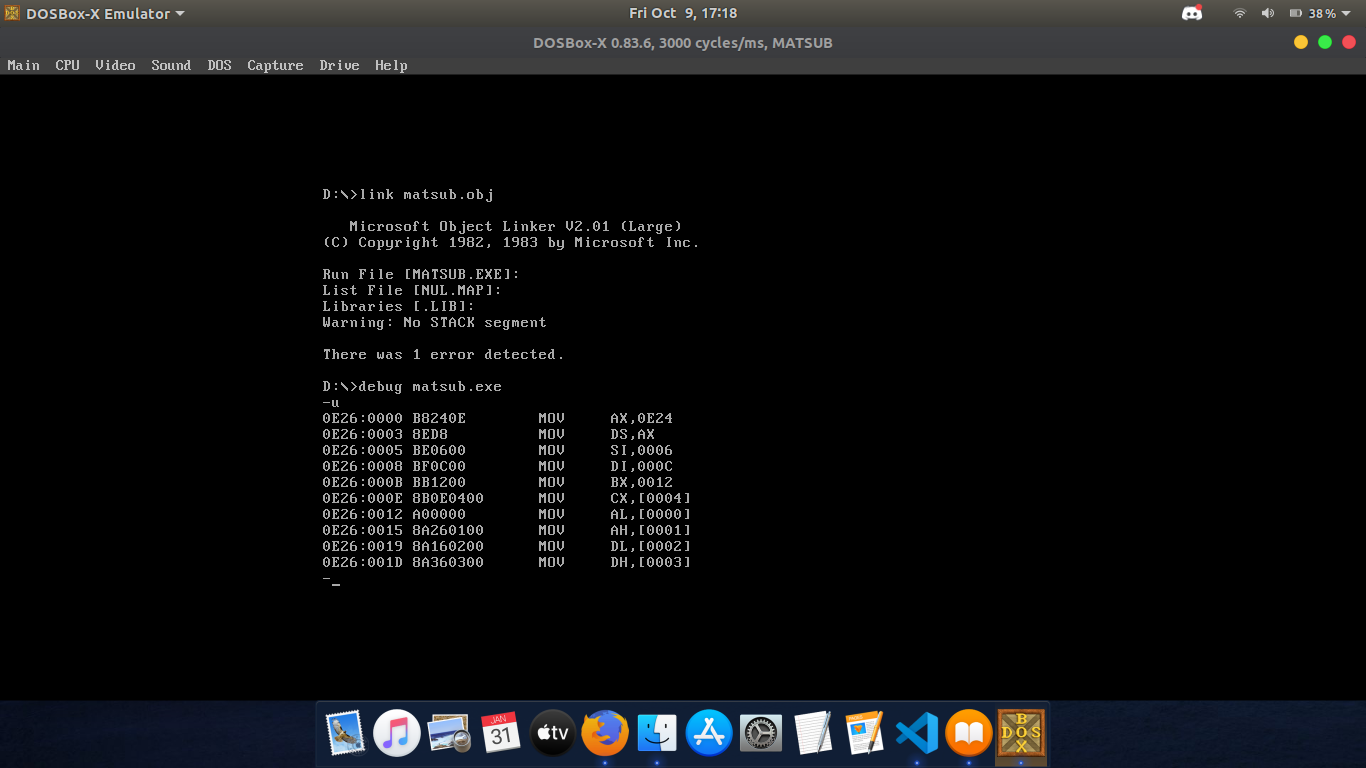
\includegraphics[trim = 100mm 60mm 200mm 120mm, clip, width = \textwidth]{Pics/MSUS.png}
\end{figure}
\subsubsection*{\textbf{Input and Output:}}
\begin{figure}[h]
    \centering
    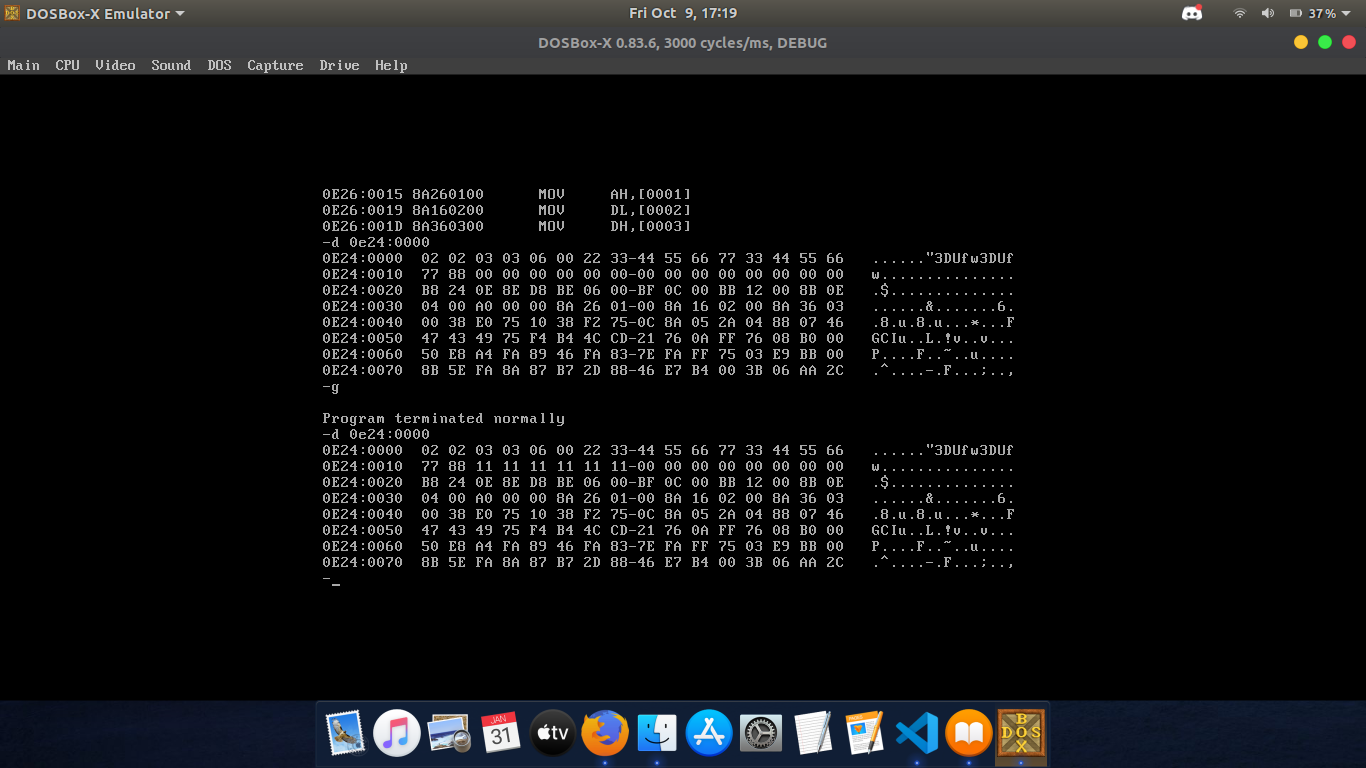
\includegraphics[trim = 100mm 60mm 100mm 80mm, clip, width = \textwidth]{Pics/MSIO.png}
    \caption{ \textbf{Input:} \emph{mat1:} 22H, 33H, 44H, 55H, 66H, 77H; \emph{mat2:} 33H, 44H, 55H, 66H, 77H, 88H ; \newline \hspace{1cm}
              \textbf{Output:} \emph{mat3:} 11H, 11H, 11H, 11H, 11H, 11H}
\end{figure}
\hrule
\subsection*{\textbf{Result:}}
The 8086 programs were written to perform matrix operations, and the results observed.
\end{flushleft}
\hrule
\newpage
%-------------------------------------------------------------------------------------------------------------------------------------------
%-------------------------------------------------------------------------------------------------------------------------------------------
% Ex 6
\begin{flushleft}
\section*{\textbf{Ex 6: Sorting Operations}}
\subsection*{\textbf{Aim:}} 
To perform sorting operations in 8086.

\vspace{1cm}
\hrule
\subsection*{\textbf{\underline{Ascending Order}}}

\subsubsection*{\textbf{Algorithm:}}
\begin{itemize}
    \item Move the data segment to the AX register and then move it to the DS register.
    \item Move value of count to CL register.
    \item Move offset of arr into SI register under label OUTER.
    \item Move value of count to CH register.
    \item Move value at [SI] to AL register, [SI+1] to AH register, under label INNER.
    \item Compare AH, AL with CMP AH, AL.
    \item If CF = 0, jump to label NOSWAP. 
    \item Swap values of AH, AL with XCHG AH, AL
    \item Move value in AL to [SI] register, AH to [SI+1].
    \item Increment SI, decrement CH under label NOSWAP.
    \item Jump to INNER if ZF = 0.
    \item Decrement CL and jump to OUTER if ZF = 0.
\end{itemize}

\newpage
\subsubsection*{\textbf{Program:}}

\begin{table}[htb]
\centering
\resizebox{\columnwidth}{!}{
\begin{tabular}{|l|l|} 
\hline
\textbf{Program}                                                 & \textbf{Comments}                             \\ 
\hline
\hline
assume cs:code, ds:data                                          & Declare code and data segments                \\
\hline
data segment                                                     & Start of data segment                         \\
\hline
arr db 05H, 04H, 03H, 02H, 01H                                   & Define array of values arr                    \\
\hline
count db 04H                                                     & Define byte count with hex value 04           \\
\hline
data ends                                                        & End of data segment                           \\
\hline
code segment                                                     & Start of code segment                         \\
\hline
start:~mov ax, data                                              & Move data to AX register                      \\
\hline
mov ds, ax                                                       & Move contents of AX register to DS register   \\
\hline
mov cl, count                                                    & Move value of count to CL register            \\
\hline
outer:~mov si, offset arr                                        & Move offset of arr to SI register             \\
\hline
mov ch, count                                                    & Move value of count to CH register            \\
\hline
inner:~mov al, [si]                                              & Move value at offset in SI to AL register     \\
\hline
mov ah, [si+1]                                                   & Move value at offset in SI register +1 to AH  \\
\hline 
cmp ah, al                                                       & Compare values in AH, AL registers            \\
\hline
jnc noswap                                                       & Jump to NOSWAP if CF = 0                      \\
\hline
xchg al, ah                                                      & Swap values in AL, AH registers               \\
\hline
mov [si], al                                                     & Move value in AL register to offset at [SI]   \\
\hline
mov [si+1], ah                                                   & Move value in AH register to offset at [SI]+1 \\
\hline
noswap:~inc si                                                   & Increment value of SI                         \\
\hline
dec ch                                                           & Decrement value of CH                         \\
\hline
jnz inner                                                        & Jump to INNER if ZF = 0                       \\
\hline
dec cl                                                           & Decrement value of CL                         \\
\hline
jnz outer                                                        & Jump to OUTER if ZF = 0                       \\
\hline
mov ah, 4ch                                                & To request interrupt                          \\
\hline
int 21h                                                          & Request interrupt routine                     \\ 
\hline
code ends                                                        & End of code segment                           \\
\hline
end start                                                        &                                               \\
\hline
\end{tabular}
}
\end{table}

\newpage
\subsection*{\textbf{Unassembled code:}}
\begin{figure}[h]
    \centering
    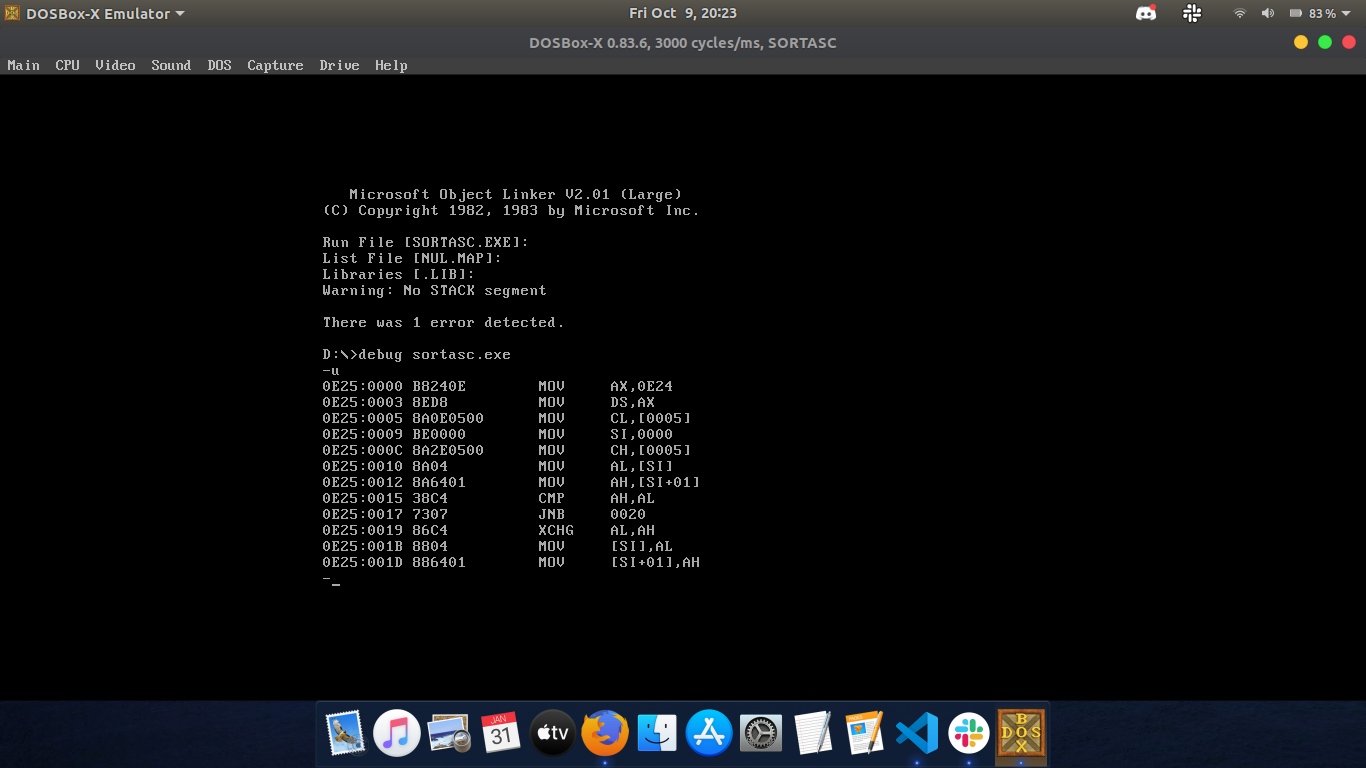
\includegraphics[trim = 100mm 60mm 200mm 120mm, clip, width = \textwidth]{Pics/SAUS.png}
\end{figure}
\subsubsection*{\textbf{Input and Output:}}
\begin{figure}[h]
    \centering
    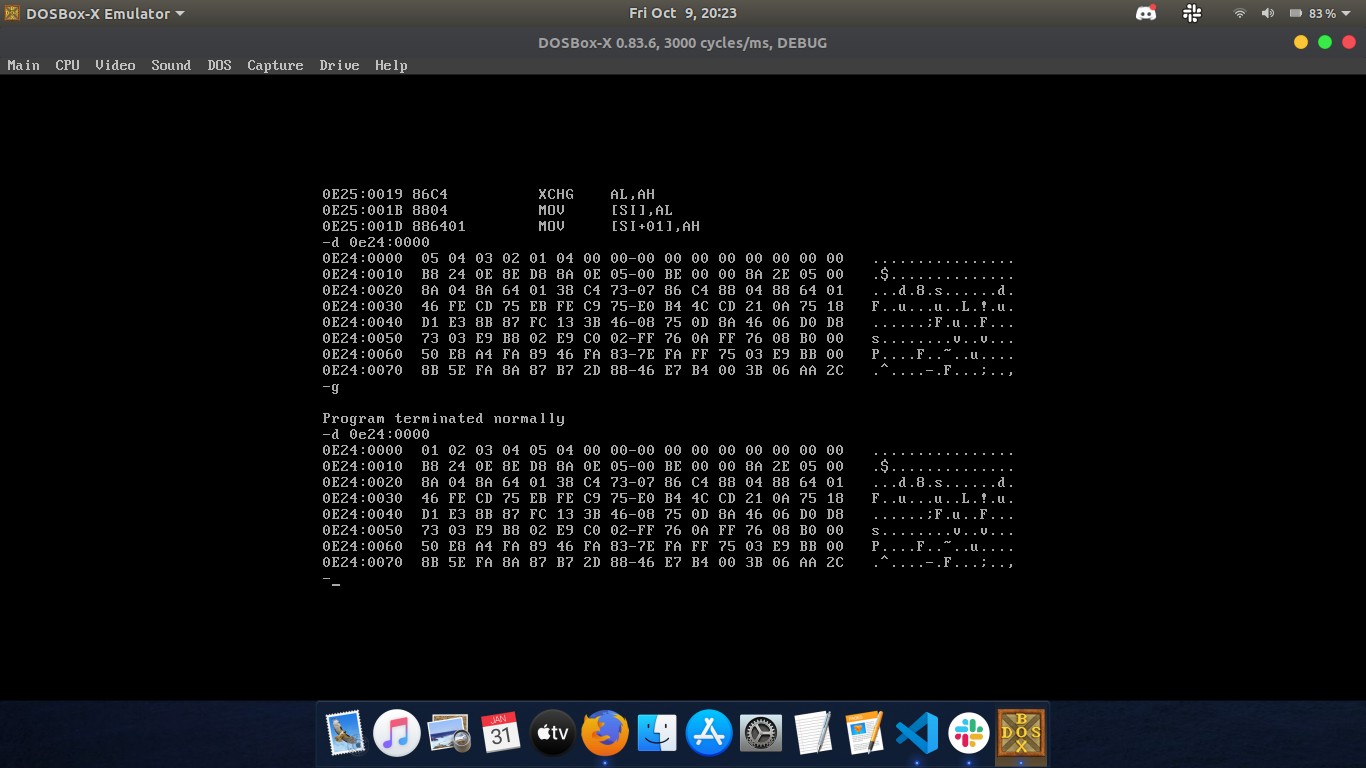
\includegraphics[trim = 100mm 60mm 100mm 80mm, clip, width = \textwidth]{Pics/SAIO.png}
    \caption{ \textbf{Input:} 05H, 04H, 03H, 02H, 01H; \newline \hspace{1cm}
              \textbf{Output:} 01H, 02H, 03H, 04H, 05H}
\end{figure}
%-------------------------------------------------------------------------------------------------------------------------------------------
\hrule
\newpage
\subsection*{\textbf{\underline{Descending Order}}}

\subsubsection*{\textbf{Algorithm:}}
\begin{itemize}
    \item Move the data segment to the AX register and then move it to the DS register.
    \item Move value of count to CL register.
    \item Move offset of arr into SI register under label OUTER.
    \item Move value of count to CH register.
    \item Move value at [SI] to AL register, [SI+1] to AH register, under label INNER.
    \item Compare AH, AL with CMP AH, AL.
    \item If CF = 1, jump to label NOSWAP. 
    \item Swap values of AH, AL with XCHG AH, AL
    \item Move value in AL to [SI] register, AH to [SI+1].
    \item Increment SI, decrement CH under label NOSWAP.
    \item Jump to INNER if ZF = 0.
    \item Decrement CL and jump to OUTER if ZF = 0.
\end{itemize}

\newpage
\subsubsection*{\textbf{Program:}}

\begin{table}[htb]
\centering
\resizebox{\columnwidth}{!}{
\begin{tabular}{|l|l|} 
\hline
\textbf{Program}                                                 & \textbf{Comments}                             \\ 
\hline
\hline
assume cs:code, ds:data                                          & Declare code and data segments                \\
\hline
data segment                                                     & Start of data segment                         \\
\hline
arr db 05H, 04H, 03H, 02H, 01H                                   & Define array of values arr                    \\
\hline
count db 04H                                                     & Define byte count with hex value 04           \\
\hline
data ends                                                        & End of data segment                           \\
\hline
code segment                                                     & Start of code segment                         \\
\hline
start:~mov ax, data                                              & Move data to AX register                      \\
\hline
mov ds, ax                                                       & Move contents of AX register to DS register   \\
\hline
mov cl, count                                                    & Move value of count to CL register            \\
\hline
outer:~mov si, offset arr                                        & Move offset of arr to SI register             \\
\hline
mov ch, count                                                    & Move value of count to CH register            \\
\hline
inner:~mov al, [si]                                              & Move value at offset in SI to AL register     \\
\hline
mov ah, [si+1]                                                   & Move value at offset in SI register +1 to AH  \\
\hline 
cmp ah, al                                                       & Compare values in AH, AL registers            \\
\hline
jc noswap                                                        & Jump to NOSWAP if CF = 1                      \\
\hline
xchg al, ah                                                      & Swap values in AL, AH registers               \\
\hline
mov [si], al                                                     & Move value in AL register to offset at [SI]   \\
\hline
mov [si+1], ah                                                   & Move value in AH register to offset at [SI]+1 \\
\hline
noswap:~inc si                                                   & Increment value of SI                         \\
\hline
dec ch                                                           & Decrement value of CH                         \\
\hline
jnz inner                                                        & Jump to INNER if ZF = 0                       \\
\hline
dec cl                                                           & Decrement value of CL                         \\
\hline
jnz outer                                                        & Jump to OUTER if ZF = 0                       \\
\hline
mov ah, 4ch                                                & To request interrupt                          \\
\hline
int 21h                                                          & Request interrupt routine                     \\ 
\hline
code ends                                                        & End of code segment                           \\
\hline
end start                                                        &                                               \\
\hline
\end{tabular}
}
\end{table}

\newpage
\subsection*{\textbf{Unassembled code:}}
\begin{figure}[h]
    \centering
    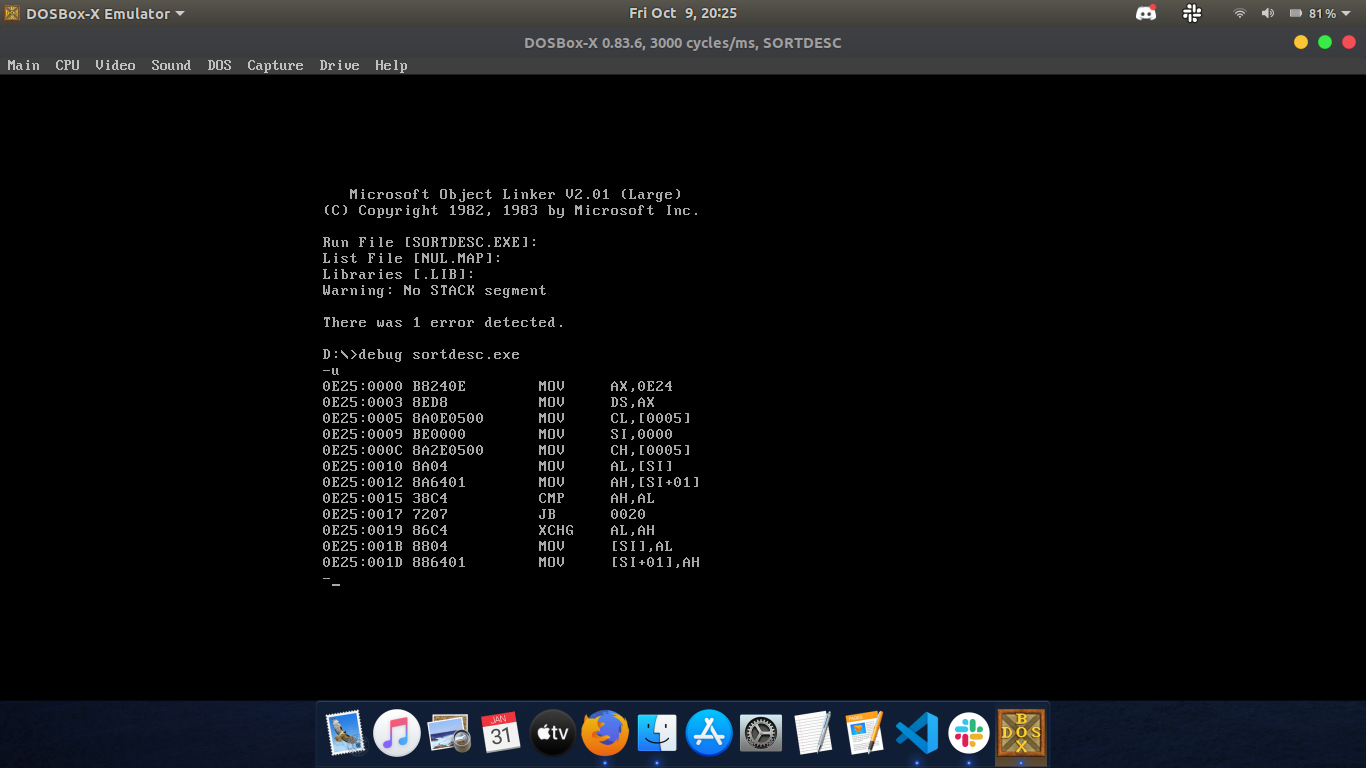
\includegraphics[trim = 100mm 60mm 200mm 120mm, clip, width = \textwidth]{Pics/SDUS.png}
\end{figure}
\subsubsection*{\textbf{Input and Output:}}
\begin{figure}[h]
    \centering
    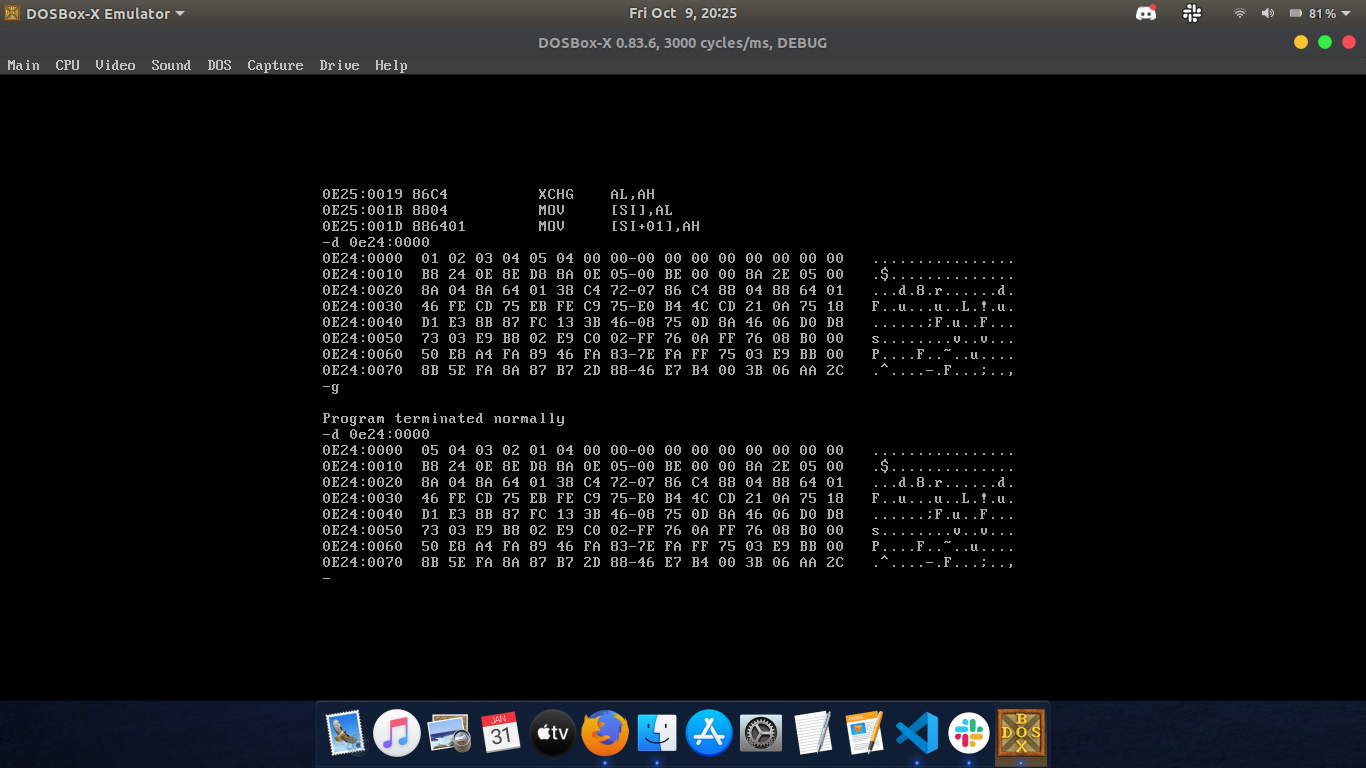
\includegraphics[trim = 100mm 60mm 100mm 80mm, clip, width = \textwidth]{Pics/SDIO.png}
    \caption{ \textbf{Input:} 01H, 02H, 03H, 04H, 05H; \newline \hspace{1cm}
              \textbf{Output:} 05H, 04H, 03H, 02H, 01H}
\end{figure}
\hrule
\subsection*{\textbf{Result:}}
The 8086 programs were written to perform matrix operations, and the results observed.
\end{flushleft}
\hrule
\newpage
%-------------------------------------------------------------------------------------------------------------------------------------------
%-------------------------------------------------------------------------------------------------------------------------------------------
% Ex 7
\begin{flushleft}
\section*{\textbf{Ex 7: BCD Addition and Subtraction}}
\subsection*{\textbf{Aim:}} 
To perform BCD addition and subtraction operations in 8086.

\vspace{1cm}
\hrule
\subsection*{\textbf{\underline{BCD Addition}}}

\subsubsection*{\textbf{Algorithm:}}
\begin{itemize}
    \item Move the data segment to the AX register and then move it to the DS register.
    \item Move value of num1 to AL, num2 to BL, carry to CL registers.
    \item Add AL and BL using ADD AL, BL.
    \item Perform Decimal Adjust After Addition using DAA instruction.
    \item Move value of AL to ans.
    \item Jump to label HERE if no carry.
    \item Increment value of CL.
    \item Move value of CL to carry, under label HERE.
\end{itemize}

\newpage
\subsubsection*{\textbf{Program:}}

\begin{table}[htb]
\centering
\resizebox{\columnwidth}{!}{
\begin{tabular}{|l|l|} 
\hline
\textbf{Program}                                                 & \textbf{Comments}                             \\ 
\hline
\hline
assume cs:code, ds:data                                          & Declare code and data segments                \\
\hline
data segment                                                     & Start of data segment                         \\
\hline
num1 db 25H                                                      & Define byte num1 with value 25                \\
\hline
num2 db 36H                                                      & Define byte num2 with value 36                \\
\hline
ans db ?                                                         & Define byte ans for result                    \\
\hline
carry db 00H                                                     & Define byte carry with value 00               \\
\hline
data ends                                                        & End of data segment                           \\
\hline
code segment                                                     & Start of code segment                         \\
\hline
start:~mov ax, data                                              & Move data to AX register                      \\
\hline
mov ds, ax                                                       & Move contents of AX register to DS register   \\
\hline
mov al, num1                                                     & Move value of num1 to AL register             \\
\hline             
mov bl, num2                                                     & Move value of num2 to BL register             \\
\hline
mov cl, carry                                                    & Move value of carry to CL register            \\
\hline 
add al, bl                                                       & AL = AL + BL                                  \\
\hline
daa                                                              & Decimal Adjust after Addition                 \\
\hline
mov ans, al                                                      & Move value of AL register into ans            \\
\hline
jnc here                                                         & Jump to label HERE if no carry                \\
\hline
inc cl                                                           & Increment value of CL                         \\
\hline
here:~mov carry, cl                                              & Move value of CL register into carry          \\
\hline
mov ah, 4ch                                                      & To request interrupt                          \\
\hline
int 21h                                                          & Request interrupt routine                     \\ 
\hline
code ends                                                        & End of code segment                           \\
\hline
end start                                                        &                                               \\
\hline
\end{tabular}
}
\end{table}

\newpage
\subsection*{\textbf{Unassembled code:}}
\begin{figure}[h]
    \centering
    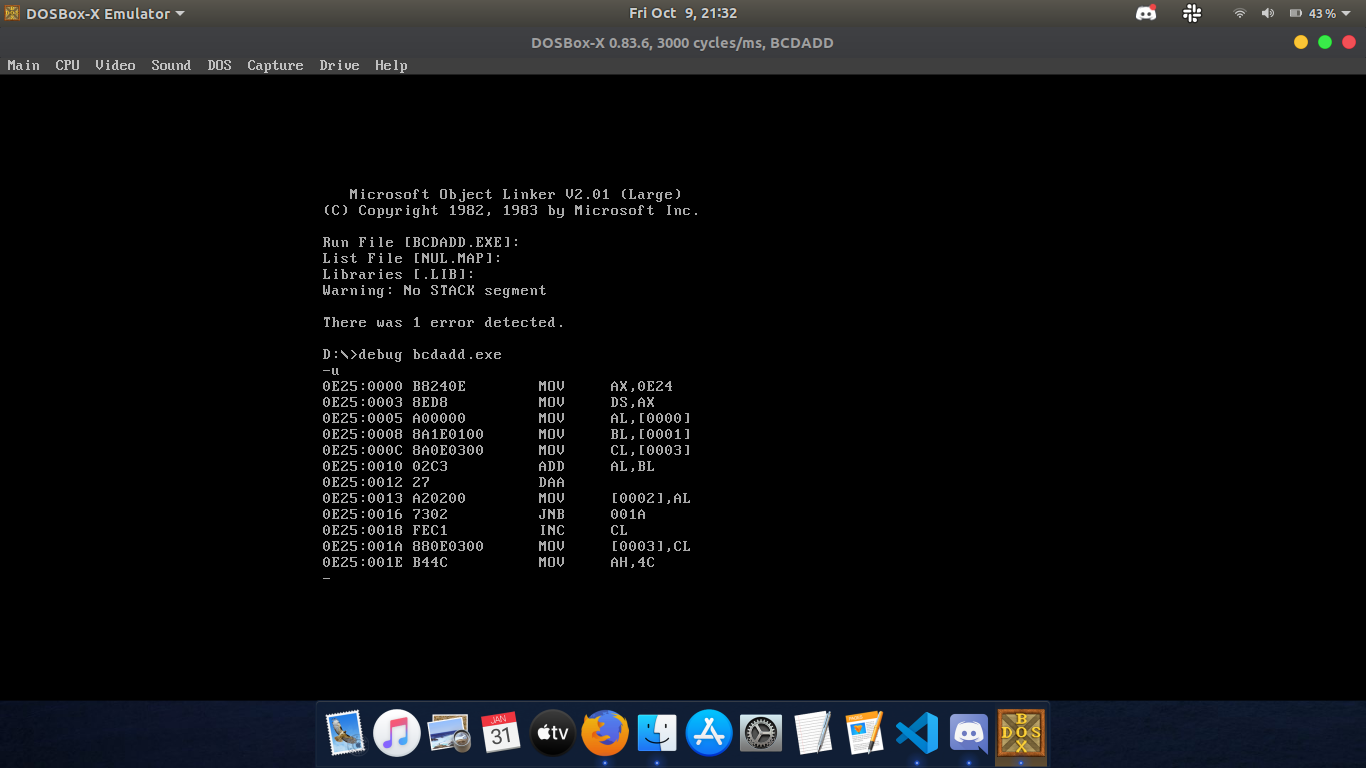
\includegraphics[trim = 100mm 60mm 200mm 120mm, clip, width = \textwidth]{Pics/BAUS.png}
\end{figure}
\subsubsection*{\textbf{Input and Output:}}
\begin{figure}[h]
    \centering
    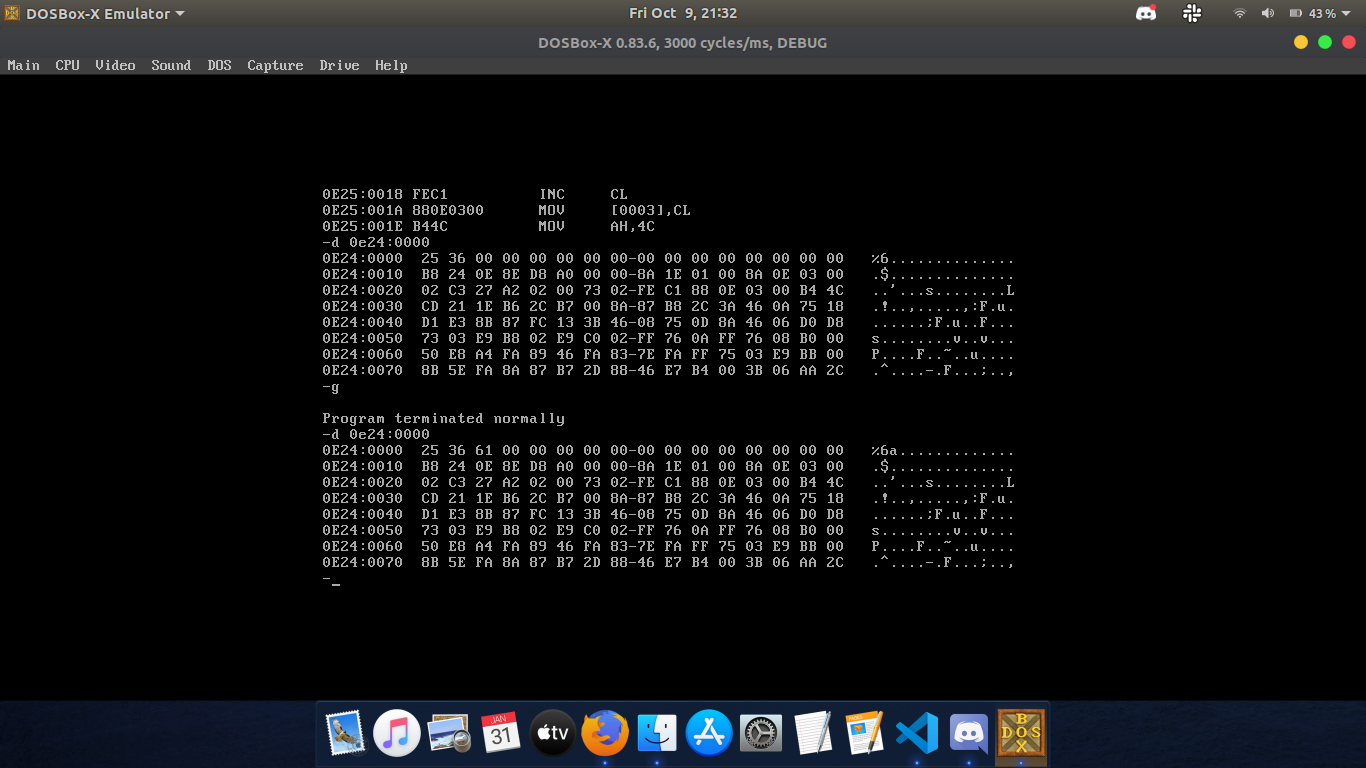
\includegraphics[trim = 100mm 60mm 100mm 80mm, clip, width = \textwidth]{Pics/BAIO.png}
    \caption{ \textbf{Input:} num1: 25, num2: 36; \newline \hspace{1cm}
                \textbf{Output:} ans: 61, carry: 0}
\end{figure}
%-------------------------------------------------------------------------------------------------------------------------------------------
\hrule
\newpage
\subsection*{\textbf{\underline{BCD Subtraction}}}

\subsubsection*{\textbf{Algorithm:}}
\begin{itemize}
    \item Move the data segment to the AX register and then move it to the DS register.
    \item Move value of num1 to AL, num2 to BL, sign to CL registers.
    \item Subtract AL and BL using SUB AL, BL.
    \item Perform Decimal Adjust After Subtraction using DAS instruction.
    \item Jump to label HERE if no carry.
    \item Move value in AL to BL register, 99H to AL register.
    \item Subtract AL and BL using SUB AL, BL.
    \item Add 1 to AL using ADD AL, 01H.
    \item Perform Decimal Adjust after Addition using DAA instruction.
    \item Increment value of CL.
    \item Move value of CL to sign, under label HERE.
    \item Move value of AL to ans.
\end{itemize}

\newpage
\subsubsection*{\textbf{Program:}}

\begin{table}[htb]
\centering
\resizebox{\columnwidth}{!}{
\begin{tabular}{|l|l|} 
\hline
\textbf{Program}                                                 & \textbf{Comments}                             \\ 
\hline
\hline
assume cs:code, ds:data                                          & Declare code and data segments                \\
\hline
data segment                                                     & Start of data segment                         \\
\hline
num1 db 25H                                                      & Define byte num1 with value 25                \\
\hline
num2 db 36H                                                      & Define byte num2 with value 36                \\
\hline
ans db ?                                                         & Define byte ans for result                    \\
\hline
sign db 00H                                                      & Define byte sign with value 00                \\
\hline
data ends                                                        & End of data segment                           \\
\hline
code segment                                                     & Start of code segment                         \\
\hline
start:~mov ax, data                                              & Move data to AX register                      \\
\hline
mov ds, ax                                                       & Move contents of AX register to DS register   \\
\hline
mov al, num1                                                     & Move value of num1 to AL register             \\
\hline             
mov bl, num2                                                     & Move value of num2 to BL register             \\
\hline
mov cl, sign                                                     & Move value of sign to CL register             \\
\hline 
sub al, bl                                                       & AL = AL - BL                                  \\
\hline
das                                                              & Decimal Adjust after Subtraction              \\
\hline                                                           
jnc here                                                         & Jump to label HERE if CF = 0                  \\
\hline
mov bl, al                                                       & Move value of AL to BL register               \\
\hline
mov al, 99H                                                      & Move hex value 99H to AL register             \\
\hline
sub al, bl                                                       & AL = AL - BL                                  \\
\hline
add al, 01H                                                      & AL = AL + 1                                   \\
\hline 
daa                                                              & Decimal Adjust after Addition                 \\
\hline
inc cl                                                           & Increment value of CL                         \\
\hline
here:~mov ans, al                                                & Move value of AL to ans                       \\
\hline
mov sign, cl                                                     & Move value of CL to sign                      \\
\hline
mov ah, 4ch                                                      & To request interrupt                          \\
\hline
int 21h                                                          & Request interrupt routine                     \\ 
\hline
code ends                                                        & End of code segment                           \\
\hline
end start                                                        &                                               \\
\hline
\end{tabular}
}
\end{table}

\newpage
\subsection*{\textbf{Unassembled code:}}
\begin{figure}[h]
    \centering
    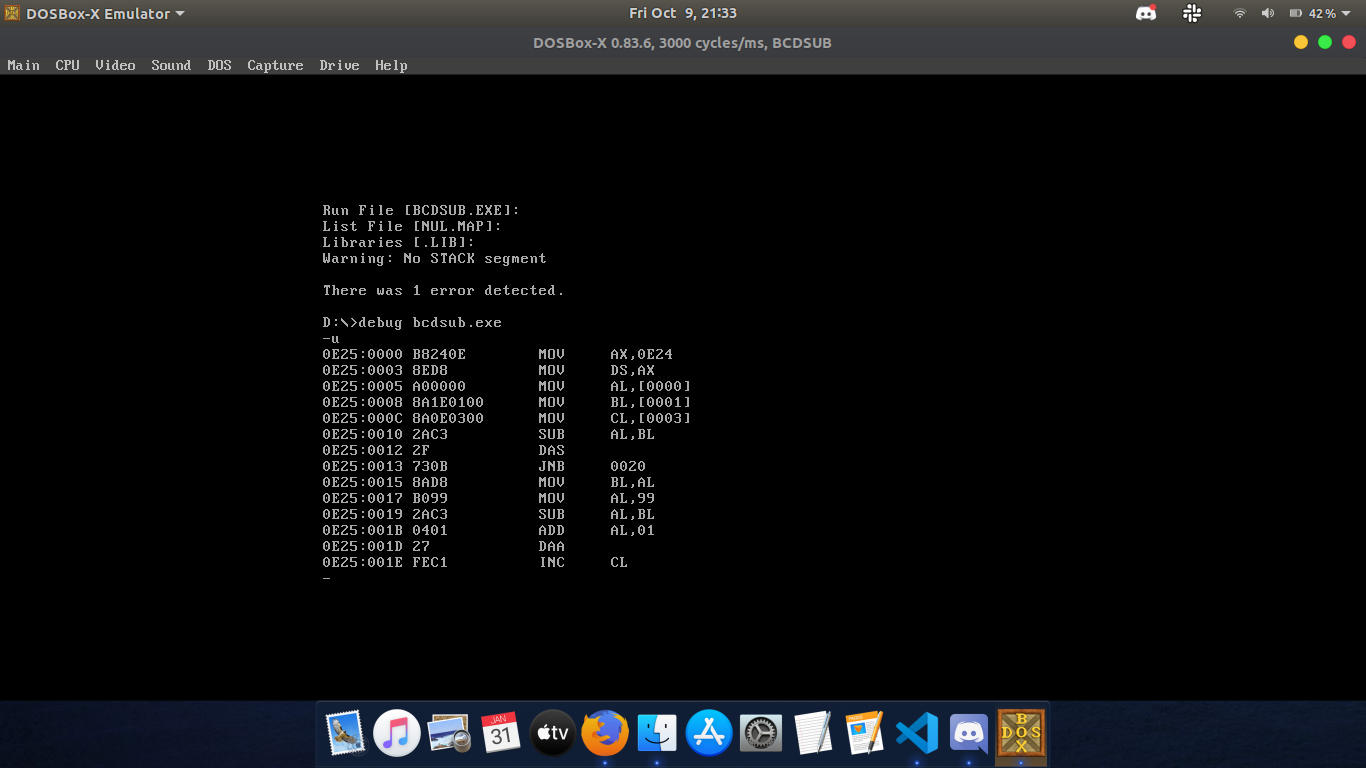
\includegraphics[trim = 100mm 60mm 200mm 120mm, clip, width = \textwidth]{Pics/BSUS.png}
\end{figure}
\subsubsection*{\textbf{Input and Output:}}
\begin{figure}[h]
    \centering
    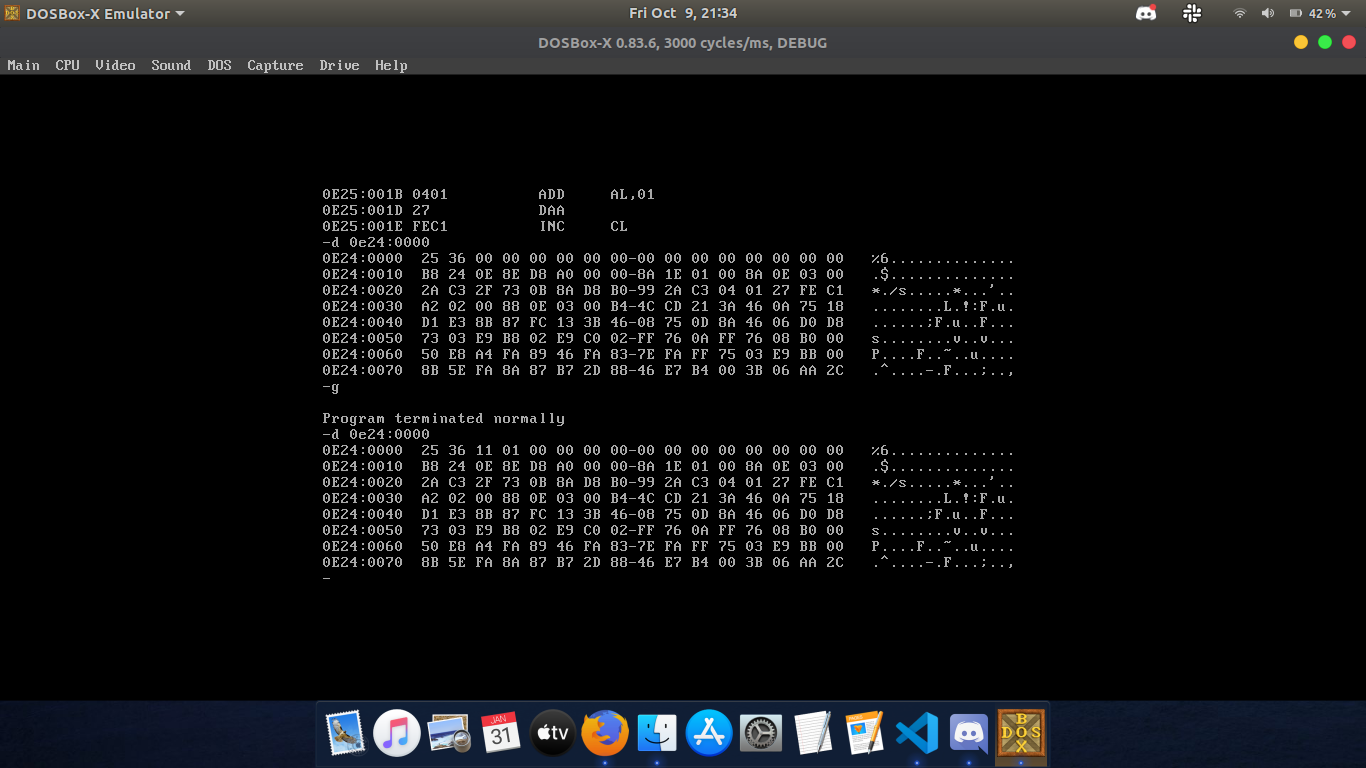
\includegraphics[trim = 100mm 60mm 100mm 80mm, clip, width = \textwidth]{Pics/BSIO.png}
    \caption{ \textbf{Input:} num1: 25, num2: 36; \newline \hspace{1cm}
                \textbf{Output:} ans: 11, sign: 1}
\end{figure}
\hrule
\subsection*{\textbf{Result:}}
The 8086 programs were written to perform BCD addition and subtraction operations, and the results observed.
\end{flushleft}
\end{document}
